\chapter{Relationship between Algorithms and Complexity}


\section{Problems and Algorithms}
The concept of a "problem" colligates a set of questions making reference to the dynamic or structural particularities of an entity- processes or objects- that acquires pinpointed, defined answers, whose accuracy can be rigorous demonstrated. The units create the universe of the problem. That segment of the problem, which is formerly familiar (known) represents the facts of the problem and the answers to the question shape the solutions. ~\cite{giumale2004introducere};
\\
Making use of a conventional inscription in order to specify an effective approach, taking into account the computational individuality of a calculus machine, it's called an \textbf{algorithm}.

An algorithm that can be accepted by a calculus machine consists of a limited amount of instructions with accurate signification, that can be implemented by the machine in a restricted period of time in order to determine the answer of a problem.

The definition of the algorithm reveals the crucial distinction between a function and an algorithm, which is, to be more specifically, the distinction between a functional representation of a problem and its effective solution. ~\cite{giumale2004introducere}

In this chapter, we will define various metrics for estimating an algorithm's performances in regard to a specific metric, such as: \textbf{RM1}, \textbf{RM2} with enhanced variations \textbf{ERM1}, \textbf{ERM2}.


\section{From algorithm to Normalized rComplexity}
Algorithms' Complexity Theory studies the static and the dynamic performances of mechanical-solvable problems. Static performances aim the clarity of the evaluated algorithm or the abstraction level imposed by used operations, while, more interesting and comparable, the dynamic performances imposes a calculus regarding the amount of resources (e.g. total execution time, peak memory usage) required for executing the algorithm. ~\cite{giumale2004introducere}; Theoretical, such metrics can be exactly calculated for any given algorithm.

\begin{remark}
    Mechanical-solvable problems inevitably makes us think to the related field in physics. An intuitive approach on the mechanical-solvable process is accessible
    to understanding when considering massive motion elements rather than transistors in technologies as advanced as 7nm.

    An example of an early mechanical solution (exhibited in 1862 at The International Exhibition in South Kensington, UK) to a mechanical-solvable problems is the Babbage's design for the difference engine, which is an automatic mechanical calculator designed to tabulate polynomial functions.

    This was a solution for approximation some mathematical functions frequently used, including logarithmic and trigonometric functions, which could be approximated by polynomials.

    \begin{figure}[H]
        \centering
        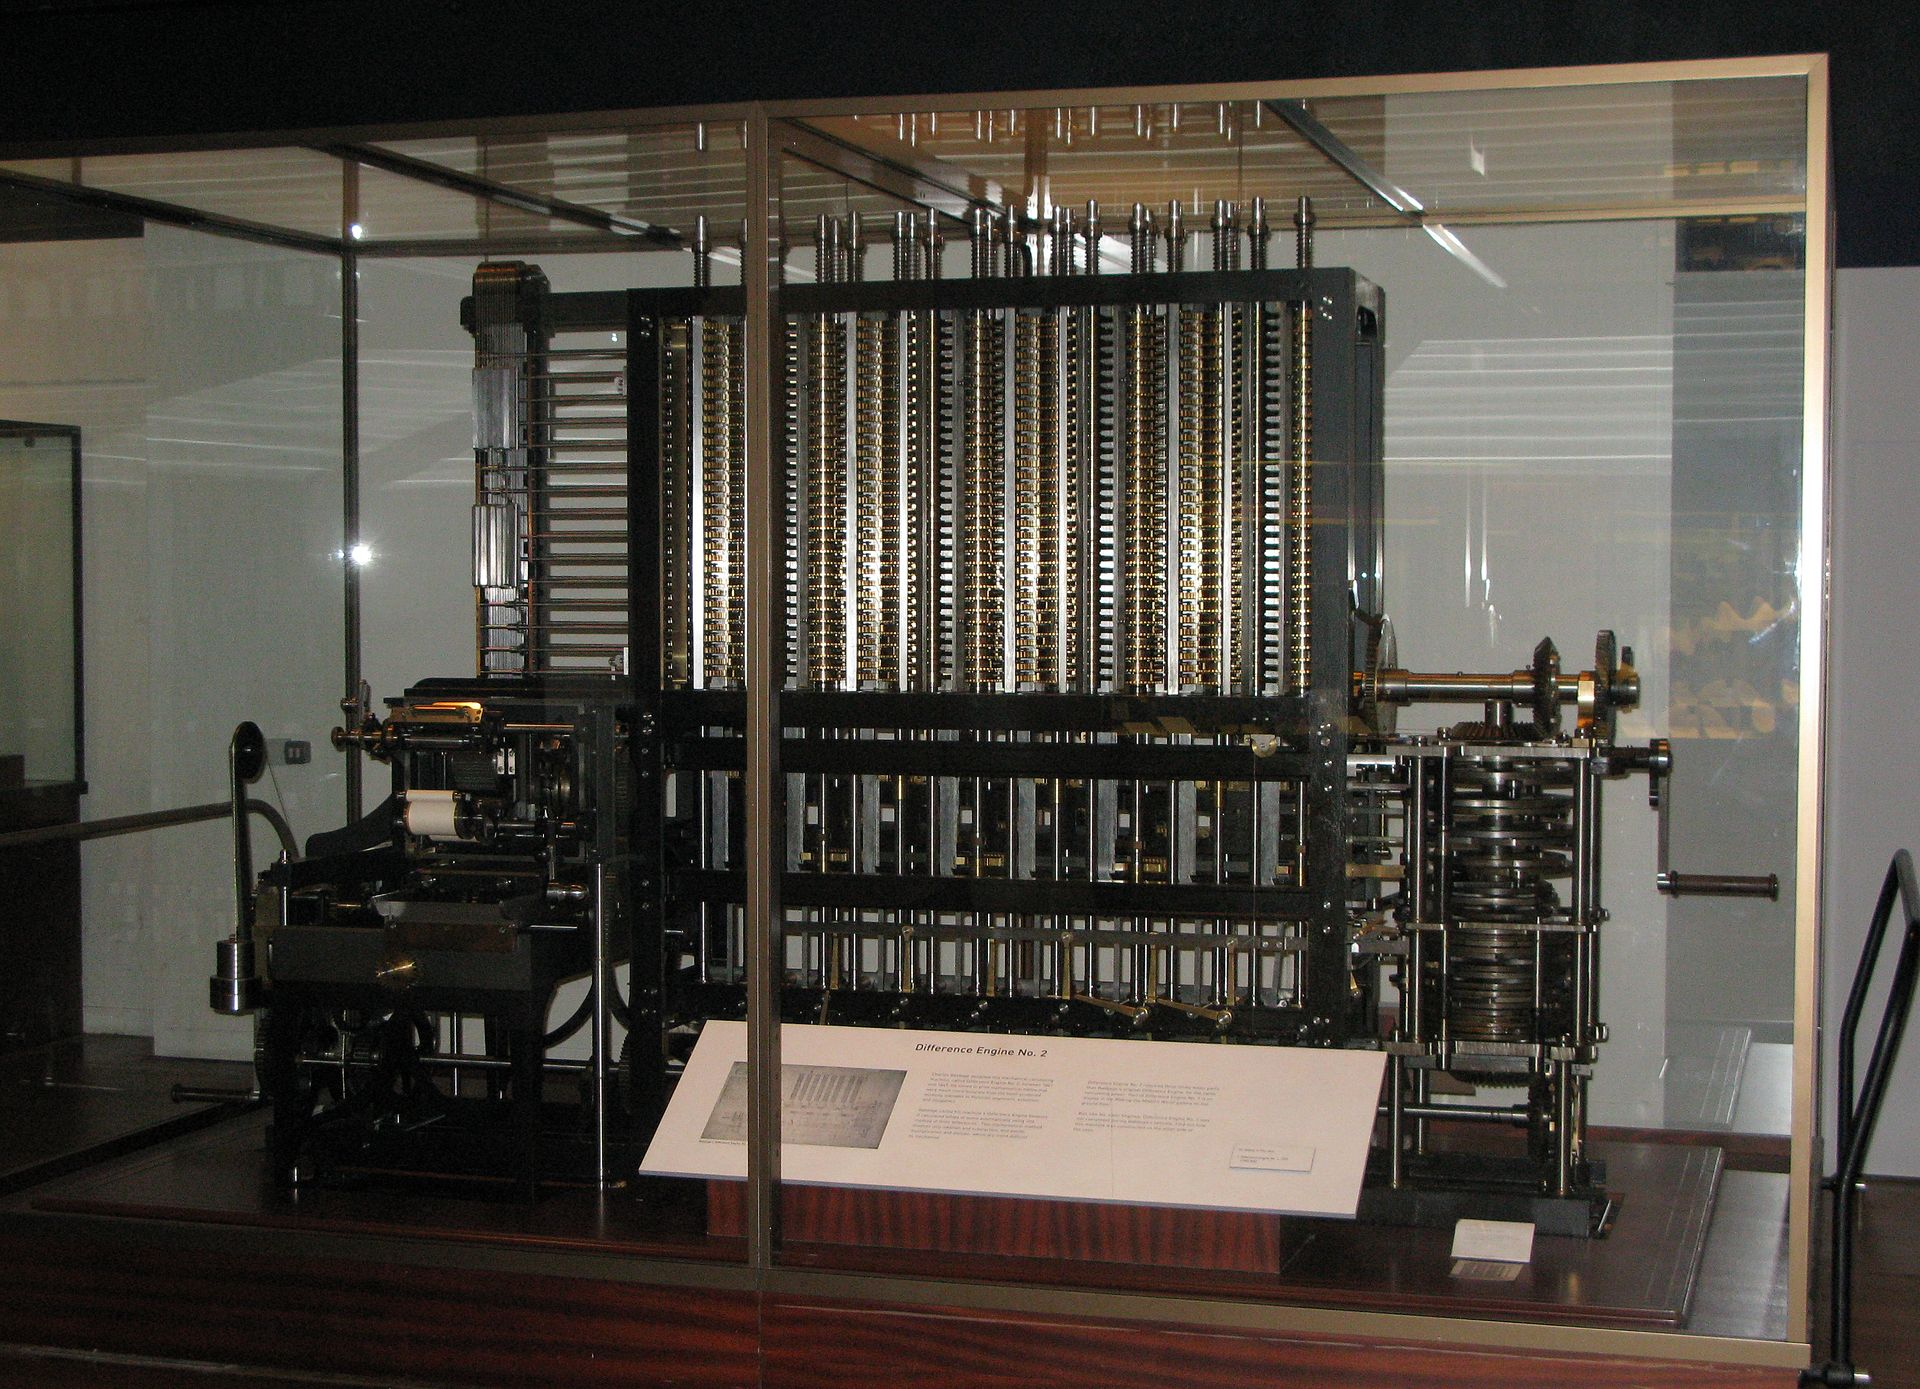
\includegraphics[width=0.5\textwidth]{BabbageDifferenceEngine}
        \caption{An implementation built from Babbage's design of a difference engine exhibited at The London Science Museum}.
    \end{figure}

\end{remark}

While the dynamic performances of an algorithm are precisely calculable, due to the high complexity (By high complexity it is denoted that it is extremely difficult to exactly compute it) of most computer programs, it is often more suitable an approximation. Such resemblance is provided by the classical model, with drastic compromise compared to the real behavior in a non-asymptotic analysis. A in-between solution for approximating the dynamic performances of an algorithm is provided by Normalized rComplexity Calculus Model, which aim to close the gap between the architecture of the computing machine and a generic-written algorithm for solving a problem.


\section{Estimating computational time based on Normalized rComplexity}
Let an arbitrary algorithm $Alg$ characterized by the complexity function $f$ with a variable input dimension $n \in \mathcal{N}^{*}$. Consider that the input size is bounded such that $n \in [n_{min}, n_{max}]$. \\
We aim to define various metrics for approximation an average computational time required based on the size of the input and the algorithm's complexity function  $T(n_{min}, n_{max})$.\\

\begin{definition}
    \textbf{RM1}

    Defined as a metric for time estimation (capable of generalization to any other estimators) based on arithmetic mean in Normalized rComplexity model is defined as follows:
    \[  T(n_{min}, n_{max}) = \dfrac{\sum\limits_{n=n_{min}}^{n_{max}} g_{1}(n)}{n_{max} - n_{min} + 1}  \]
\end{definition}

\begin{definition}
    \textbf{RM2}

    Defined as a metric for time estimation (capable of generalization to any other estimators) based on Mean-Value Theorem(Lagrange) using integrals in Normalized rComplexity model is defined as follows:
    \[  T(n_{min}, n_{max}) = \dfrac{\int\limits_{n_{min}}^{n_{max}} g_{1}(n) dn}{n_{max} - n_{min}}  \]
\end{definition}

The previous two metrics are tailored for systems where the input size is bounded but there is no additional knowledge regarding the weights and probabilities of occurrence. If this information is available, we can redefine the previous metrics using the acquisition data.

\begin{definition}
    \textbf{ERM1}, an enhanced metric for time estimation based on arithmetic mean in Normalized rComplexity model is defined as follows:
    \[  T(n_{min}, n_{max}) = \sum\limits_{n=0}^{f} p_{n} \cdot g_{1}(n + n_{min})  \]
    where:
    \begin{itemize}
        \item $p_{0}$ is the weight associated with $n_{0} = n_{min}$
        \item $p_{1}$ is the weight associated with $n_{1} = n_{min + 1}$
        \item $p_{f}$ is the weight associated with $n_{f} = n_{max}$
    \end{itemize}
    and $f = max - min + 1$.
\end{definition}

\begin{definition}
    \textbf{ERM2}, an enhanced metric for time estimation based on Mean-Value Theorem(Lagrange) using integrals in Normalized rComplexity model is defined as follows:
    \[  T(n_{min}, n_{max}) =\sum\limits_{k=0}^{f-1} p_{k} \cdot \int\limits_{n_{k}}^{n_{k+1}} g_{1}(n) dn  \]
    where:
    \begin{itemize}
        \item $p_{0}$ is the weight associated with the probability of the input to be bounded in the interval $[n_{0}, n_{1}]$
        \item $p_{1}$ is the weight associated with the probability of the input to be bounded in the interval $[n_{1}, n_{2}]$
        \item $p_{f-1}$ is the weight associated with the probability of the input to be bounded in the interval $[n_{f-1}, n_{f}]$
    \end{itemize}
    and $f = max - min + 1$, and $n_{0} = n_{min}, n_{f} = n_{max}$.
\end{definition}


\section{Comparing algorithms asymptotic performances}


This section aims to compare two generic Algorithms ($Alg1$, $Alg2$) time-based performances based on associated Big r-Theta class from Normalized rComplexity model, by asymptotically correlating the characterized complexity functions $f, f'$.

For specific application of this theoretical work, please refer to the following chapter.

Let $f \in \Theta_{1}(g_{1}(n))$ and $f' \in \Theta_{1}(g'_{1}(n))$.
We can therefore compare the time-based performances of the two algorithms by evaluating:  \[\lim_{n\to\infty} \dfrac{g_{1}(n)}{g'_{1}(n)}\]

\begin{remark}
    \[\lim_{n\to\infty} \dfrac{g_{1}(n)}{g'_{1}(n)} = \lim_{n\to\infty} \dfrac{f(n)}{f'(n)}\]
\end{remark}

\begin{definition}
    Let $f \in \Theta_{1}(g_{1}(n))$ and $f' \in \Theta_{1}(g'_{1}(n))$. $f$ is part of a smaller class than $f'$ iff $\lim_{n\to\infty} \dfrac{g_{1}(n)}{g'_{1}(n)} = 0$.
\end{definition}
\begin{lemma}
    If  $ \lim_{n\to\infty} \dfrac{g_{1}(n)}{g'_{1}(n)} = 0 $ , then $Alg1$ will terminate faster than $Alg2$ for any input size $n \geq n_{0}$, with the possibility of computing $n_{0} \in \mathcal{N}^{*}$.
\end{lemma}
\begin{proof}
    $\lim_{n\to\infty} \dfrac{g_{1}(n)}{g'_{1}(n)} = 0 \Rightarrow g_{1}(n) < g'_{1}(n)\ \forall n \geq n_{0} \Rightarrow f(n) < f'(n) \ \forall n \geq n_{0}'$
\end{proof}

\begin{definition}
    Let $f \in \Theta_{1}(g_{1}(n))$ and $f' \in \Theta_{1}(g'_{1}(n))$. $f$ is part of the same class as $f'$ iff $\lim_{n\to\infty} \dfrac{g_{1}(n)}{g'_{1}(n)} = r$ and $r \in \mathcal{R}_{+}$.
    If $f$ is part of the same class as $f'$, we can distinguish the following cases:
    $$
    \lim_{n\to\infty} \dfrac{g_{1}(n)}{g'_{1}(n)} =
    \begin{cases}
        x \in (0,1), f\ has\ a\ smaller\ constant\ than\ f' \\
        1, f\ has\ the\ same\ constant\ as\ f'\\
        y \in (1,\infty), f\ has\ a\ bigger\ constant\ than\ f'
    \end{cases}
    $$
\end{definition}

\begin{lemma}
    If  $ \lim_{n\to\infty} \dfrac{g_{1}(n)}{g'_{1}(n)} = r \in (0,1) $ , then $Alg1$ will terminate faster than $Alg2$ for any input size $n \geq n_{0}$, with the possibility of computing $n_{0} \in \mathcal{N}^{*}$.
\end{lemma}
\begin{proof}
    $\lim_{n\to\infty} \dfrac{g_{1}(n)}{g'_{1}(n)} < 1 \Rightarrow g_{1}(n) < g'_{1}(n)\ \forall n \geq n_{0} \Rightarrow f(n) < f'(n) \ \forall n \geq n_{0}'$
\end{proof}

\begin{lemma}
    If  $ \lim_{n\to\infty} \dfrac{g_{1}(n)}{g'_{1}(n)} = r \in (1,\infty) $ , then $Alg1$ will terminate slower than $Alg2$ for any input size $n \geq n_{0}$, with the possibility of computing $n_{0} \in \mathcal{N}^{*}$.
\end{lemma}
\begin{proof}
    $\lim_{n\to\infty} \dfrac{g_{1}(n)}{g'_{1}(n)} > 1 \Rightarrow g_{1}(n) > g'_{1}(n)\ \forall n \geq n_{0} \Rightarrow f(n) > f'(n) \ \forall n \geq n_{0}'$
\end{proof}



\begin{definition}
    Let $f \in \Theta_{1}(g_{1}(n))$ and $f' \in \Theta_{1}(g'_{1}(n))$. $f$ is part of a bigger class than $f'$ iff $\lim_{n\to\infty} \dfrac{g_{1}(n)}{g'_{1}(n)} = \infty$.
\end{definition}
\begin{lemma}
    If  $ \lim_{n\to\infty} \dfrac{g_{1}(n)}{g'_{1}(n)} = \infty $ , then $Alg1$ will terminate slower than $Alg2$ for any input size $n \geq n_{0}$, with the possibility of computing $n_{0} \in \mathcal{N}^{*}$.
\end{lemma}
\begin{proof}
    $\lim_{n\to\infty} \dfrac{g_{1}(n)}{g'_{1}(n)} = \infty \Rightarrow g_{1}(n) > g'_{1}(n)\ \forall n \geq n_{0} \Rightarrow f(n) > f'(n) \ \forall n \geq n_{0}'$
\end{proof}


\section{Comparing algorithms interval-based performances}
Comparing algorithms asymptotic performances based on Normalized rComplexity was a generic way of comparing two algorithms' asymptotic performances for unbounded large input. However, asymptotic performance is not always relevant for computer programs that have a settled \textit{(or a interval-based approximation, with or without weights on sub-specific intervals)} range of input size in order of solving a specific task.
\\ Consider an application responsible of scheduling a football league agenda for the next competitive season, avoiding conflicts and following specific objectives. This problem can be modeled and solved as a \textit{constraint satisfaction problem}(CSP) with different flavors. An asymptotic performance analyzer would simply pick the lowest complexity function in consideration to asymptotic behavior. However, the application is not designed to run on extremely large input size, as the cardinal of the set of all teams part of a football league is a bounded well-known small integer (\textit{most leagues have between 14 and 20 teams}). Therefore, it may be a wise choice to have another method of comparing different algorithms with respect to finite upper bounded input.

For a fixed unique input size $n_{0}\in \mathcal{N}^{*}$, we can use the following natural comparison:
\begin{lemma}
    If  $ \lim_{n\to n_{0}} \dfrac{g_{1}(n)}{g'_{1}(n)} = \dfrac{g_{1}(n_{0})}{g'_{1}(n_{0})} = r \in [0,1) $ , then $Alg1$ will terminate faster than $Alg2$ for the input size $n_{0}$.
\end{lemma}
Symmetrical:
\begin{lemma}
    If  $ \lim_{n\to n_{0}} \dfrac{g_{1}(n)}{g'_{1}(n)} = \dfrac{g_{1}(n_{0})}{g'_{1}(n_{0})} = r \in (1,\infty) $ , then $Alg2$ will terminate faster than $Alg1$ for the input size $n_{0}$.
\end{lemma}
\begin{remark}
    If  $ \lim_{n\to n_{0}} \dfrac{g_{1}(n)}{g'_{1}(n)} = \dfrac{g_{1}(n_{0})}{g'_{1}(n_{0})} = 1$, rComplexity calculus considers $Alg1$ and $Alg2$ equivalent from a computational cost-based perspective.
\end{remark}

For a bounded interval-based input size $n \in [n_{min}, n_{max}]$, we can use the following comparison based on the metrics determined in the previous sections:

\begin{theorem}
    If $ \dfrac{T_{1}(n_{min}, n_{max})}{T_{2}(n_{min}, n_{max})} = r \in [0,1) $ , then $Alg1$ will terminate faster (in average) than $Alg2$ for a randomly distribution of input size $n \in [n_{min}, n_{max}]$, assuming \[T_{1}(n_{min}, n_{max}) = \dfrac{\sum\limits_{n=n_{min}}^{n_{max}} g_{1}(n)}{n_{max} - n_{min} + 1}\] and \[T_{2}(n_{min}, n_{max}) = \dfrac{\sum\limits_{n=n_{min}}^{n_{max}} g'_{1}(n)}{n_{max} - n_{min} + 1}\] where $Alg1$ has a complexity function associated to the normalized rComplexity Big 1-Theta defined by $g_{1}$ and $Alg2$ has a complexity function associated to the normalized rComplexity Big 1-Theta defined by $g'_{1}$.
\end{theorem}

\begin{corollary}
    If $ \dfrac{T_{1}(n_{min}, n_{max})}{T_{2}(n_{min}, n_{max})} = r \in (1,\infty) $ , then $Alg2$ will terminate faster (in average) than $Alg1$ for a randomly distribution of input size $n \in [n_{min}, n_{max}]$.
\end{corollary}

\begin{remark}
    If  $ \dfrac{T_{1}(n_{min}, n_{max})}{T_{2}(n_{min}, n_{max})} = 1$, rComplexity calculus considers $Alg1$ and $Alg2$ equivalent from a computational cost-based perspective for a randomly distribution of input size $n \in [n_{min}, n_{max}]$.
\end{remark}

\begin{remark}
    If  $ \dfrac{T_{1}(n_{min}, n_{max})}{T_{2}(n_{min}, n_{max})} = 1$, a tiebreak can be done by a deep analysis of the less dominant features as described in the Enhanced rComplexity model feature extraction in the next chapter.
\end{remark}

\begin{remark}
    Theorem stands likewise using Mean-Value Theorem(Lagrange), with
    \[  T_{1}(n_{min}, n_{max}) = \dfrac{\int\limits_{n_{min}}^{n_{max}} g_{1}(n) dn}{n_{max} - n_{min}}  \]
    \[  T_{2}(n_{min}, n_{max}) = \dfrac{\int\limits_{n_{min}}^{n_{max}} g'_{1}(n) dn}{n_{max} - n_{min}}  \]
    for a randomly distribution of input size $n \in [n_{min}, n_{max}]$.
\end{remark}

Currently, we assumed that the input size is randomly distributed in a bounded interval. Further information about the probabilistic distribution of input size $n \in [n_{min}, n_{max}]$ can offer more insights to this complexity model and a refined comparison model can be established.

\begin{theorem}
    If $ \dfrac{T_{1}(n_{min}, n_{max})}{T_{2}(n_{min}, n_{max})} = r \in [0,1) $ , then $Alg1$ will terminate faster (in average) than $Alg2$ for a probabilistic distribution of input size $n \in [n_{min}, n_{max}]$, assuming


    \[T_{1}(n_{min}, n_{max}) = \sum\limits_{n=0}^{f} p_{n} \cdot g_{1}(n + n_{min})\] and \[T_{2}(n_{min}, n_{max}) = \sum\limits_{n=0}^{f} p_{n} \cdot g'_{1}(n + n_{min})\] where $Alg1$ has a complexity function associated to the normalized rComplexity Big 1-Theta defined by $g_{1}$ and $Alg2$ has a complexity function associated to the normalized rComplexity Big 1-Theta defined by $g'_{1}$, and

    \begin{itemize}
        \item $p_{0}$ is the weight associated with $n_{0} = n_{min}$
        \item $p_{1}$ is the weight associated with $n_{1} = n_{min + 1}$
        \item $p_{f}$ is the weight associated with $n_{f} = n_{max}$
    \end{itemize}
    with $f = max - min + 1$.

\end{theorem}

\begin{corollary}
    If $ \dfrac{T_{1}(n_{min}, n_{max})}{T_{2}(n_{min}, n_{max})} = r \in (1,\infty) $ , then $Alg2$ will terminate faster (in average) than $Alg1$ for a probabilistic distribution of input size $n \in [n_{min}, n_{max}]$.
\end{corollary}

\begin{remark}
    If  $ \dfrac{T_{1}(n_{min}, n_{max})}{T_{2}(n_{min}, n_{max})} = 1$, rComplexity calculus considers $Alg1$ and $Alg2$ equivalent from a computational cost-based perspective for probabilistic distribution of input size $n \in [n_{min}, n_{max}]$.
\end{remark}

\begin{remark}
    Theorem stands likewise using Mean-Value Theorem(Lagrange), with :
    \[  T_{1}(n_{min}, n_{max}) =\sum\limits_{k=0}^{f-1} p_{k} \cdot \int\limits_{n_{k}}^{n_{k+1}} g_{1}(n) dn  \]
    \[  T_{2}(n_{min}, n_{max}) =\sum\limits_{k=0}^{f-1} p_{k} \cdot \int\limits_{n_{k}}^{n_{k+1}} g'_{1}(n) dn  \]
    for a probabilistic distribution of input size $n \in [n_{min}, n_{max}]$, where:
    \begin{itemize}
        \item $p_{0}$ is the weight associated with the probability of the input to be bounded in the interval $[n_{0}, n_{1}]$
        \item $p_{1}$ is the weight associated with the probability of the input to be bounded in the interval $[n_{1}, n_{2}]$
        \item $p_{f-1}$ is the weight associated with the probability of the input to be bounded in the interval $[n_{f-1}, n_{f}]$
    \end{itemize}
    and $f = max - min + 1$, and $n_{0} = n_{min}, n_{f} = n_{max}$.

\end{remark}